\documentclass[conference]{IEEEtran}
\IEEEoverridecommandlockouts
% The preceding line is only needed to identify funding in the first footnote. If that is unneeded, please comment it out.
\usepackage{cite}
\usepackage{amsmath,amssymb,amsfonts}
\usepackage{tabularx,booktabs}
\usepackage{algorithmic}
\usepackage{bm}      % for "\bm" macro
\usepackage{graphicx}
\usepackage{textcomp}
\usepackage{float}
\usepackage{xcolor}

\def\BibTeX{{\rm B\kern-.05em{\sc i\kern-.025em b}\kern-.08em
    T\kern-.1667em\lower.7ex\hbox{E}\kern-.125emX}}
\begin{document}

\title{Traffic Flow Optimization Using Quantum Annealer}

\author{\IEEEauthorblockN{Dhaval Patel}
\IEEEauthorblockA{\textit{Department Of Computer Science} \\
\textit{University of Maryland Baltimore County}\\
up08495@umbc.edu}
\and
\IEEEauthorblockN{Aarsh Oza}
\IEEEauthorblockA{\textit{Department Of Computer Science} \\
\textit{University of Maryland Baltimore County}\\
aoza1@umbc.edu}
}

\maketitle

\begin{abstract}
Nowadays the main problem for commuters is the congestion on the streets. There are a few other problems that are caused due to traffic like pollution and increased fuel consumption. In this project, we have approached the given problem using the upcoming next big thing that is the Quantum Annealers. Here, we show how the traffic congestion problem can be formulated as QUBO (Quadratic Unconstrained Binary Optimization) problem. Due to some constraint of accessing the D-wave and reducing the complexity of the project, we formulated our own small case scenarios and data set where on a predefined track, number of cars having the same source and destination are allocated different routes based on the congestion on a particular route. We have designed a cost function that we penalize based on the number of vehicles that are already existing on a route. Using the cost function, we designed our main Objective function.

\end{abstract}
\vspace{6pt}
\begin{IEEEkeywords}
traffic, optimization, quantum annealers
\end{IEEEkeywords}

\section{Introduction}
As we know, there are 2 approaches in Quantum Annealing. The first being Ising Hamiltonian and the second one is Quadratic Unconstrained Binary Optimization also known as QUBO.\vspace{6pt}

\begin{figure}[ht]
\centerline{\includegraphics[width=8cm]{Ising.png}}
\caption{Equation of Ising Hamiltonian}
\label{fig}
\end{figure}

As shown in figure 1 for Ising Hamiltonian equation "h" corresponds to linear coefficient of qubit bias, while "j" corresponds to the quadratic or coupling coefficient also called strength.\vspace{6pt}

\begin{figure}[ht]
\centerline{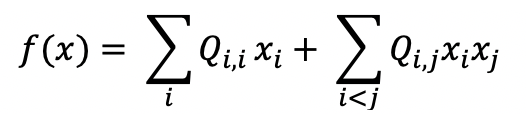
\includegraphics[width=8cm]{qubo.png}}
\caption{Equation of QUBO}
\label{fig}
\end{figure}

On the flip side the figure 2 for  QUBO deals with a matrix Q which is an upper triangular matrix. The elements on primary diagonals are linear bias while all other non zero elements are quadratic biases.\vspace{6pt}

Though Ising Hamiltonain and QUBO are Isomorphic, meaning they are convertible to one another, we decided to model our problem on QUBO formulation. There are two major reasons for formulating the problem on QUBO. They are:
\begin{itemize}
    \item The importance of the binary rule i.e. \(x^2= x\) in QUBO, because QUBO uses (0,1) binary variables and Ising Hamiltonian uses (-1,1) spin variables.\vspace{6pt}
    \item We can Represent the matrix efficiently in QUBO.
\end{itemize}

\section{Method}
To formulate the traffic flow problem, we have made an assumption that all the cars start along at the same time from location A with the goal to reach location B. We have created a data set that is similar to Microsoft's T trajectory data set of more than 1000 cars. Another assumption is made that each car requires an equal amount of time to traverse any particular street segment. The next step is data preprocessing.

\subsection{Data pre-processing on a Classical computer}
The data set is parsed to find out congestions on the streets. Another dataset with all possible routes for a car is created based on the current and destination location of that car. Based on all available alternative routes, each car is assigned with 4 alternative routes. The next step would be to formulate the minimization problem for QUBO.



\subsection{Minimizing problem}
The main goal in solving QUBO is minimizing this objective function. In simple words it means minimizing \( x^T \cdot Q \cdot x \)

\begin{figure}[ht]
\centerline{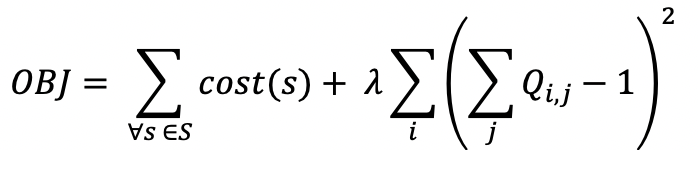
\includegraphics[width=8cm]{objective.png}}
\caption{Objective Equation}
\label{fig}
\end{figure}

The objective function consists of 2 things:\vspace{6pt}
\begin{itemize}
    \item Cost function
    \item Constraint
\end{itemize}
\vspace{6pt}
What is the cost function ?\vspace{6pt}
\newline
We already know 2 things, firstly congestion occurs when more number of cars share the same route segment. Like if more numbers of cars are present on segment s0 at same time it will create congestion on s0 street segment. Congestion is a quadratic function of the number of cars. We need a measure to penalize this situation where more cars exist on the same segment. Below is the cost function.\vspace{6pt}

\begin{figure}[ht]
\centerline{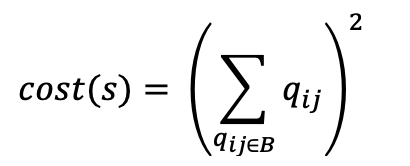
\includegraphics[width=8cm]{cost.png}}
\caption{Cost Equation}
\label{fig}
\end{figure}
What are Constraints?\vspace{6pt}
\newline
We define a binary variable having value from \{0,1\}, \( \textit{Q} _{ij} \) for every possible assignment of car to route where i represents car and j represents route. As each car can only exist in one route at a time, exactly one variable per car must be true in the minimizing of the QUBO, We define a constraint in such a way that every car is required to take exactly one route. In other words we can state that the square of summation of all variables for each distinct car i should sum up to 1. We do this procedure for every car to get the constraint in totally for every car over every possible route.
\vspace{6pt}

\begin{figure}[ht]
\centerline{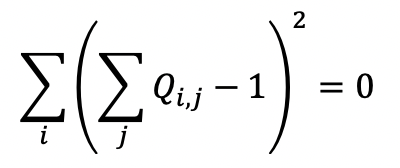
\includegraphics[width=8cm]{constraint.png}}
\caption{Constraint Equation}
\label{fig}
\end{figure}

\subsection{Rules to form the Q matrix}

There are 2 rules to form this matrix:
\begin{itemize}
    \item For every car i with possible route j, we add (−k) to the diagonal of Q given by index I(qij).\newline
In simple terms we just add -k to all diagonal terms.\vspace{6pt}

\item For every quadratic term arising from the constraint equation, we add (2k) to the corresponding off-diagonal term.
\end{itemize}
\vspace{6pt}

\subsection{Qbsolve}

Qbsolve is a library directly provided by the Dwave. The use of Qbsolve is to break a bigger problem that requires very high number qubits into a smaller problem which Quantum annealer can handle easily.


\section{Naive Example to explain the case}

We formed a naive case at first for solving traffic optimization problems to better understand the underlying mechanics of forming QUBO matrices. We modeled the naive case for 2 cars and assigned 3 routes for each car in order to create a simple case to understand.\vspace{6pt}

\begin{figure}[ht]
\centerline{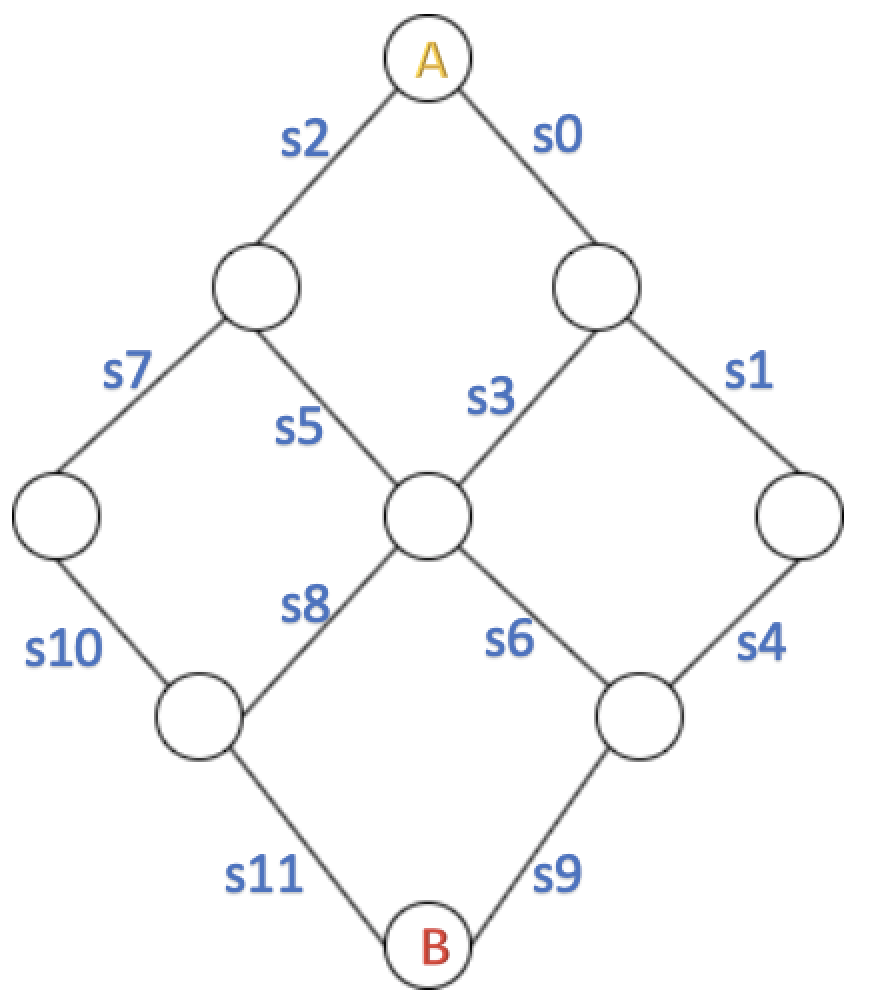
\includegraphics[width=6cm]{graph.png}}
\caption{The street network graph}
\label{fig}
\end{figure}

As shown in the figures, all the nodes represent a junction where ‘A’ is the starting point and ‘B’ is the destination. Also \( \textit{S} _{i} \) represents street segments and many such street segments combine to form a route.\vspace{6pt}

Here, we assume that both cars start at around the same time from ‘A’ with a goal to reach ‘B’. Thereafter we assigned one current route to each car:\vspace{6pt}

\begin{itemize}
    \item Car1: [s0,s3,s6,s9]
    \item Car2: [s0,s3,s8,s11]
\end{itemize}
\vspace{6pt}

We also assigned some routes each car can take:
\begin{table}[H]
\renewcommand{\arraystretch}{1.3}
\caption{Cars and Routes}
\label{Cars and Routes}
\centering
\begin{tabular}{c|c|c|c}
    \hline
    Cars  &  Route 1  &  Route 2  &  Route 3\\
    \hline
    \hline

    A  &  [s0,s3,s6,s9] (current)  &  [s0,s3,s8,s11]  &  [s2,s7,s10,s11]\\
    \hline

    B  &  [s0,s3,s6,s9]  &  [s0,s3,s8,s11] (current)  &  [s2,s7,s10,s11]\\
    \hline
\end{tabular}
\end{table}

\subsection{Cost}

We then calculated the cost for every segment from equation 4 and found the following values for all segments:

\begin{table}[H]
\renewcommand{\arraystretch}{1.3}
\caption{Cost of segments}
\label{Cost of segments}
\centering
\begin{tabular}{c|c|c}
    \hline
    Street Segment  &  Associated Cost Function  &  Value\\
    \hline
    \hline

    s0  &   (\textit{Q}_{11} + \textit{Q}_{12} + \textit{Q}_{21} + \textit{Q}_{22})^2  &  4\\
    \hline

    s3  &  (\textit{Q}_{11} + \textit{Q}_{12} + \textit{Q}_{21} + \textit{Q}_{22})^2  &  4\\
    \hline
    
    s6  &  (\textit{Q}_{11} + \textit{Q}_{21})^2  &  1\\
    \hline
    
    s9  &  (\textit{Q}_{11} + \textit{Q}_{21})^2  &  1\\
    \hline
    
    s8  &  (\textit{Q}_{12} + \textit{Q}_{22})^2  &  1\\
    \hline
    
    s11  &  (\textit{Q}_{12} + \textit{Q}_{22} + \textit{Q}_{13} + \textit{Q}_{23})^2  &  1\\
    \hline
    
    s2  &  (\textit{Q}_{13} + \textit{Q}_{23})^2  &  0\\
    \hline
    
    s7  &  (\textit{Q}_{13} + \textit{Q}_{23})^2  &  0\\
    \hline
    
    s10  &  (\textit{Q}_{13} + \textit{Q}_{23})^2  &  0\\
    \hline
\end{tabular}
\end{table}

\subsection{Constraint}

After getting cost for each segment, the next step is to form the constraint that each car cannot travel through more than one route at the same time. We form the constraint as explained in equation shown in Fig 5.\vspace{6pt}

The next and main step is to form the Q matrix which we formed by following the above mentioned rules from section of Rules given above.\vspace{6pt}

Finally after getting the matrix, the final step is to get a dot product of  \( x^T \cdot Q \cdot x \) on a Quantum Annealing Sampler. \vspace{6pt}

At last we get values for all the variables that minimize all this
dot product in turn reducing the congestion over the street network shown in fig 6.


\section{Result}

To evaluate the QUBO formulation of our traffic problem, we designed a small experiment of 100 cars. We iterated over the same data set for 50 times. For each iteration, we randomly assigned each car with 4 alternative routes.The main goal of this experiment was to map a real world problem to Quantum Annealer and finally suggest some better routes than classical algorithms.\vspace{6pt}

I wouldn’t say that the results were optimal but they were good enough to reduce the traffic by almost 300 percent. For example, we had 100 cars and 4 routes, so the optimal result would be 25 cars on each route, but on an average we got a distribution such as [24, 23, 33, 20] for each route.

\begin{figure}[H]
\centerline{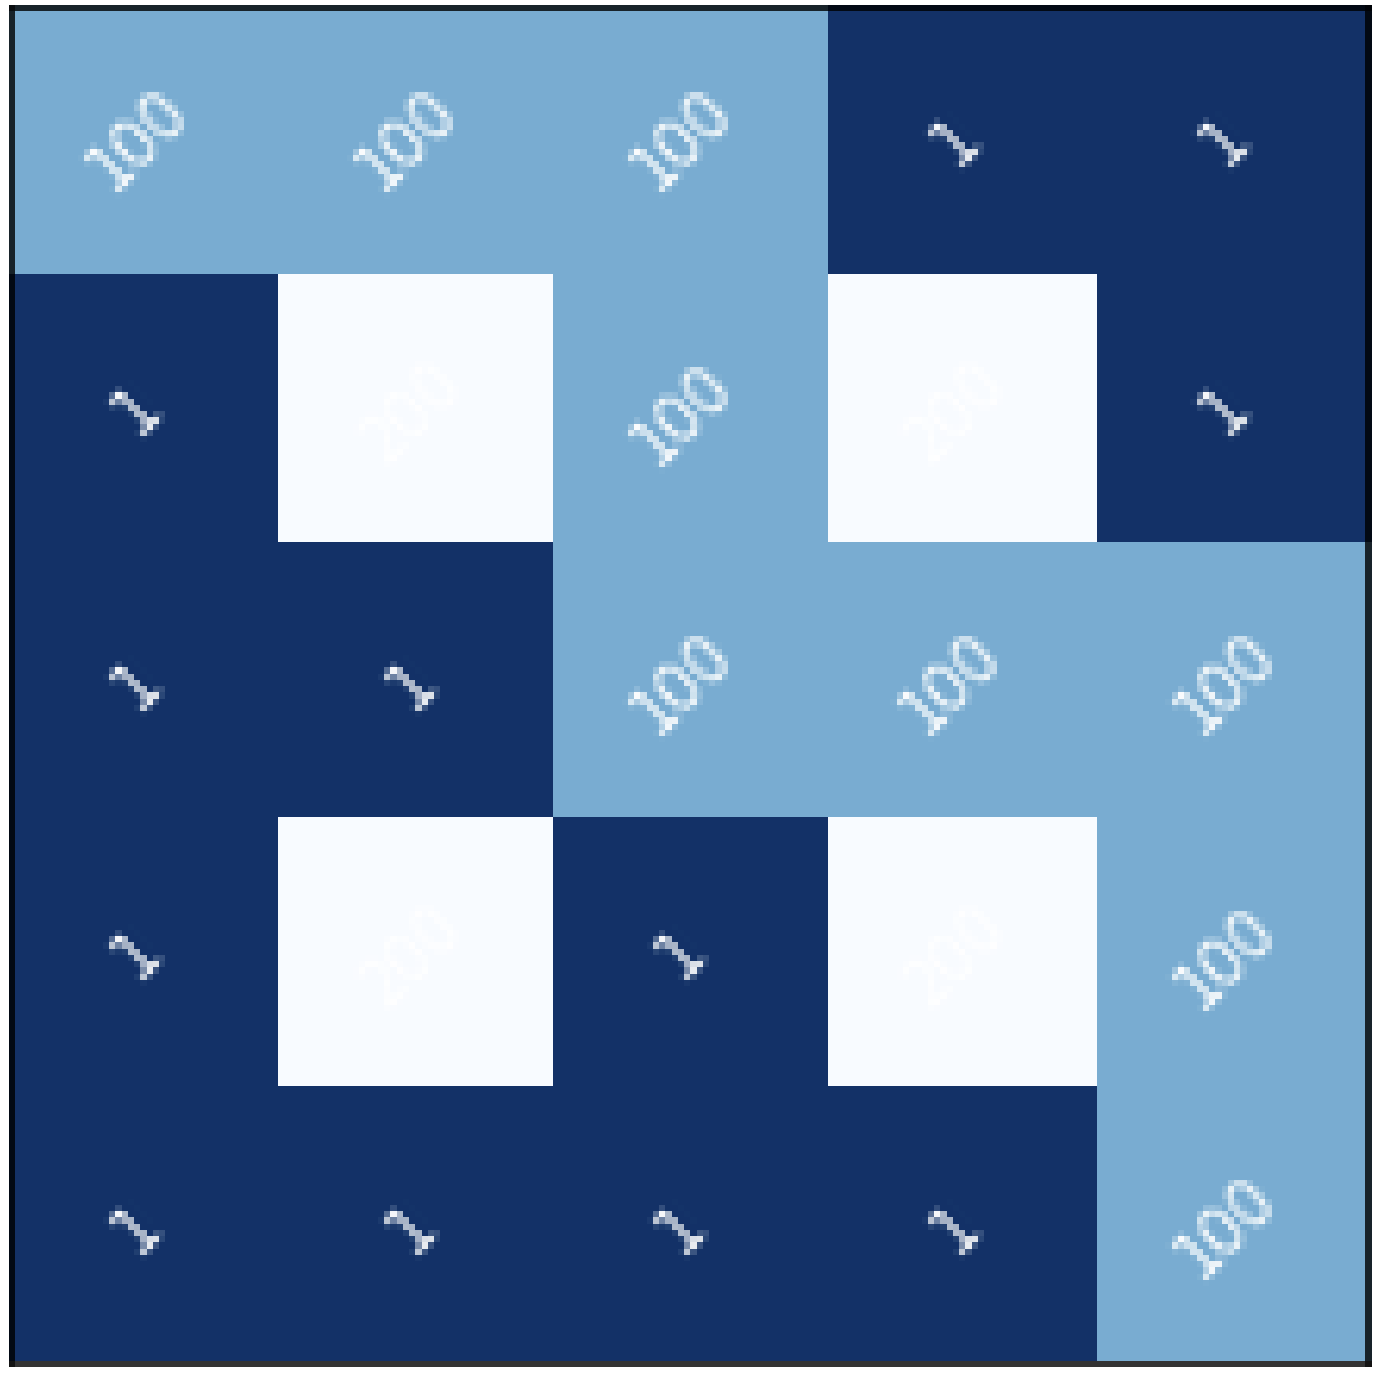
\includegraphics[width=4cm,angle=-45,origin=c]{heatmap1.png}}
\caption{Heatmap before optimizing congestion}
\label{fig}
\end{figure}

Above is the heat map for 100 cars following the same routes generated based on the classical path search algorithm such as BFS and DFS, and below is the the image for distribution of cars based on the output generated from qbsolv.

\begin{figure}[H]
\centerline{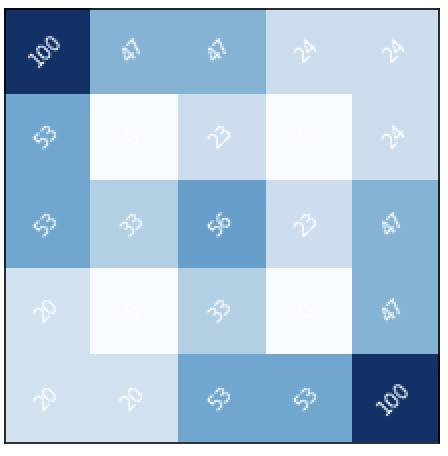
\includegraphics[width=4cm,angle=-45,origin=c]{heatmap2.png}}
\caption{Heatmap after optimizing congestion}
\label{fig}
\end{figure}

\section{Conclusion and Future work}

We have presented a highly simplified form of the very bigger and a complex problem that needs to be addressed. As we have made some assumptions like all cars starting at the same time from point A, in future we can incorporate real time location tracking using GPS for updated coordinates of the car every 5 seconds. We can also add features for communicating to infrastructures such as traffic signals.

\begin{thebibliography}{00}
\bibitem{b1} F. Neukart, G. Compostella, C. Seidel, D. V. Dollen, S. Yarkoni, and B. Parney, “Traffic Flow Optimization Using a Quantum Annealer,” Frontiers in ICT, vol. 4, 2017.

\end{thebibliography}
\vspace{12pt}


\end{document}
